\documentclass[a4paper,14pt]{extreport}
\usepackage[T2A]{fontenc}
\usepackage[utf8]{inputenc}
\usepackage[main=russian,english]{babel}
\usepackage{tempora}                % Шрифт, близкий к Times New Roman
\usepackage[a4paper,left=30mm,right=15mm,top=20mm,bottom=20mm]{geometry}
\setlength{\parindent}{1.25cm}
\renewcommand{\baselinestretch}{1.5}
\usepackage{amsmath,amssymb,graphicx,here,enumitem,caption,titlesec,tocloft,
hyperref,listings,xcolor,inconsolata, indentfirst}

% =============================================================================
% GOST 6.1.1: Поля, шрифт, интервал, отступ настроены выше
% =============================================================================

% GOST 6.2.1, 6.2.3: Заголовки структурных элементов без номера, прописные, по центру, без точки
\titleformat{\chapter}[block]
  {\centering\normalfont\Large\bfseries}{}{0pt}{\MakeUppercase}
\titlespacing*{\chapter}{0pt}{0pt}{20pt}

% Заголовки разделов: с абзацного отступа, жирные, с прописной, без точки
\titleformat{\section}
  {\normalfont\large\bfseries}{\thesection}{1em}{}
\titlespacing*{\section}{\parindent}{*2}{*1}

\titleformat{\subsection}
  {\normalfont\normalsize\bfseries}{\thesubsection}{1em}{}
\titlespacing*{\subsection}{\parindent}{*2}{*1}

% Убираем точки после номеров
\renewcommand{\thesection}{\arabic{section}}
\renewcommand{\thesubsection}{\thesection.\arabic{subsection}}
\renewcommand{\thechapter}{} % Структурные элементы не нумеруются

% =============================================================================
% GOST 6.13: Оформление содержания
% =============================================================================
\renewcommand{\cftchapfont}{\normalfont\large\bfseries}
\renewcommand{\cftchappagefont}{\normalfont\large\bfseries}
\renewcommand{\cftchapaftersnum}{} % Без точки после структурных элементов
\renewcommand{\cftsecaftersnum}{}   % Без точки после номеров разделов
\renewcommand{\cftchapleader}{\cftdotfill{\cftdotsep}}
\setlength{\cftsecindent}{2em}
\setlength{\cftsubsecindent}{4em}

% =============================================================================
% GOST 6.5, 6.6: Подписи рисунков и таблиц
% =============================================================================
\captionsetup[figure]{labelsep=endash, position=bottom, justification=raggedright, singlelinecheck=false, font=normalsize}
\captionsetup[table]{labelsep=endash, position=top, justification=raggedright, singlelinecheck=false, font=normalsize}
\renewcommand{\figurename}{Рисунок}
\renewcommand{\tablename}{Таблица}
\graphicspath{{fig/}}

% Нумерация иллюстраций и таблиц в пределах раздела (двухуровневая: 2.1, а не 2.1.1)
\counterwithin{figure}{section}
\counterwithin{table}{section}

% =============================================================================
% Оформление листингов кода
% =============================================================================
\lstset{
  inputencoding=utf8,
  extendedchars=false,
  keepspaces=true,
  language=Python,
  basicstyle=\footnotesize\ttfamily,
  numbers=left,
  numberstyle=\tiny\ttfamily,
  stepnumber=1,
  numbersep=5pt,
  backgroundcolor=\color{white},
  showspaces=false,
  showstringspaces=false,
  showtabs=false,
  frame=single,
  tabsize=2,
  captionpos=t,
  breaklines=true,
  postbreak=\raisebox{0ex}[0ex][0ex]{\ensuremath{\color{red}\hookrightarrow\space}},
  escapeinside={\%*}{*)},
  inputpath=listings,
  %% 👇 ОБЯЗАТЕЛЬНОЕ ДОБАВЛЕНИЕ ДЛЯ КИРИЛЛИЦЫ В UTF-8
  literate=
    {а}{{а}}1 {б}{{б}}1 {в}{{в}}1 {г}{{г}}1 {д}{{д}}1 {е}{{е}}1 {ё}{{ё}}1
    {ж}{{ж}}1 {з}{{з}}1 {и}{{и}}1 {й}{{й}}1 {к}{{к}}1 {л}{{л}}1 {м}{{м}}1
    {н}{{н}}1 {о}{{о}}1 {п}{{п}}1 {р}{{р}}1 {с}{{с}}1 {т}{{т}}1 {у}{{у}}1
    {ф}{{ф}}1 {х}{{х}}1 {ц}{{ц}}1 {ч}{{ч}}1 {ш}{{ш}}1 {щ}{{щ}}1 {ъ}{{ъ}}1
    {ы}{{ы}}1 {ь}{{ь}}1 {э}{{э}}1 {ю}{{ю}}1 {я}{{я}}1
    {А}{{А}}1 {Б}{{Б}}1 {В}{{В}}1 {Г}{{Г}}1 {Д}{{Д}}1 {Е}{{Е}}1 {Ё}{{Ё}}1
    {Ж}{{Ж}}1 {З}{{З}}1 {И}{{И}}1 {Й}{{Й}}1 {К}{{К}}1 {Л}{{Л}}1 {М}{{М}}1
    {Н}{{Н}}1 {О}{{О}}1 {П}{{П}}1 {Р}{{Р}}1 {С}{{С}}1 {Т}{{Т}}1 {У}{{У}}1
    {Ф}{{Ф}}1 {Х}{{Х}}1 {Ц}{{Ц}}1 {Ч}{{Ч}}1 {Ш}{{Ш}}1 {Щ}{{Щ}}1 {Ъ}{{Ъ}}1
    {Ы}{{Ы}}1 {Ь}{{Ь}}1 {Э}{{Э}}1 {Ю}{{Ю}}1 {Я}{{Я}}1
}
\renewcommand{\lstlistingname}{Листинг}
\captionsetup[lstlisting]{labelsep=endash, position=top, justification=raggedright}

% =============================================================================
% GOST 6.3.1, 6.3.2: Нумерация страниц
% =============================================================================
\usepackage{fancyhdr}
\pagestyle{fancy}
\fancyhf{}
\cfoot{\thepage}
\renewcommand{\headrulewidth}{0pt}
\renewcommand{\thepage}{\arabic{page}}

% Титульный лист считается первой страницей, но номер не ставится
\makeatletter
\patchcmd{\@makechapterhead}{\@chapapp\space\thechapter}{\@chapapp}{}{}
\makeatother

\begin{document}

% =============================================================================
% ТИТУЛЬНЫЙ ЛИСТ (GOST 5.1, 6.10)
% =============================================================================
\begin{titlepage}
\centering
{\normalsize Министерство науки и высшего образования Российской Федерации\par}
{\normalsize ФГАОУ ВО «Санкт-Петербургский политехнический университет Петра Великого»\par}
{\normalsize Институт компьютерных наук и кибербезопасности\par}
\vspace{1cm}
{\Large\bfseries ОТЧЕТ О КУРСОВОЙ РАБОТЕ\par}
\vspace{0.5cm}
{\large по теме: «Архиватор LZ77»\par}
\vspace{0.5cm}
{\normalsize по дисциплине «Структуры данных»\par}
\vspace{2cm}
\begin{flushright}
{\normalsize Выполнили: студент гр. 5151003/50001\par}
{\normalsize Гордиенков З. Ю.\par}
{\normalsize студент гр. 5151003/50001\par}
{\normalsize Мотуш В. Р.\par}
{\normalsize студент гр. 5151003/50001\par}
{\normalsize Ходос М. В.\par}
\vspace{0.5cm}
{\normalsize Руководитель: ассистент\par}
{\normalsize Грибков Н. А.\par}
\end{flushright}
\vfill
{\large Санкт-Петербург 2026\par}
\end{titlepage}

\setcounter{page}{2}
\tableofcontents
\newpage

\chapter*{ВВЕДЕНИЕ}
\addcontentsline{toc}{chapter}{ВВЕДЕНИЕ}

В ходе выполнения данной курсовой работы была создана программа-архиватор MZ77
под ОС на основе проектов GNU/Linux. Для реализации графического интерфейса
применялась графическая библиотека GTK-4.0, для работы с многопоточностью
использовалась POSIX-библиотека pthread. Также использовались заголовочные
файлы glibc:
\begin{itemize}[leftmargin=*, label={--}]
	\item stdlib.h --- выделение динамической памяти;
	\item stdio.h --- форматирование строк;
	\item string.h --- работа со строками;
	\item limits.h --- макрос максимальной длины пути;
	\item stdatomic.h --- типы и функции для безопасной работы с данными,
		доступными из параллельных потоков;
	\item stdbool.h --- определение типа данных bool.
\end{itemize}
Для разработки применялась система сборки autotools (autoconf 2.72, automake
1.17), система контроля версий git 2.47.3, хостинг проектов github.com .

Целью работы было создание простого в использовании архиватора с
удовлетворительным коэффициентом сжатия.
\newpage

\chapter*{ОПИСАНИЕ ПО}
\addcontentsline{toc}{chapter}{ОПИСАНИЕ ПО}
\begin{figure}[H]
  \centering
  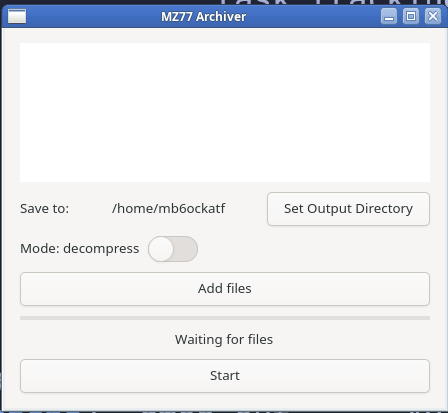
\includegraphics[width=0.8\textwidth]{pic/window.png}
\caption{\centering Окно архиватора}
  \label{fig:window}
\end{figure}
После запуска программы на экране появляется окно graphical tool kit. В нём
можно выбрать \textit{исходные файлы}, режим работы (сжатие либо распаковка),
целевую директорию -- место, куда будут помещены результаты работы.
\begin{figure}[H]
  \centering
  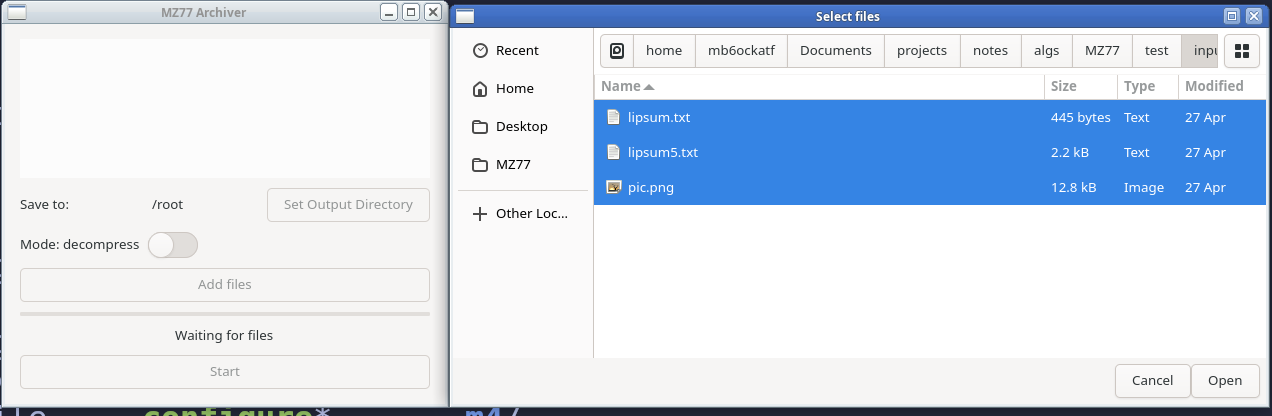
\includegraphics[width=1\textwidth]{pic/choose_window.png}
\caption{\centering Окно выбора исходных файлов.}
  \label{fig:choosewindow}
\end{figure}

По завершению работы архиватор закрывается автоматически.

\newpage
\chapter*{ИСПОЛЬЗУЕМЫЕ СТРУКТУРЫ ДАННЫХ}
\addcontentsline{toc}{chapter}{ИСПОЛЬЗУЕМЫЕ СТРУКТУРЫ ДАННЫХ}

Список выбранных исходных файлов сохраняется в виде очереди. Очередь
прикреплена к state-объекту AppData, объект очереди --- TaskItem. Определение
очереди доступно в приложении B.

Адреса строк в окне просмотра хранятся в хэш-таблице мощностью 65536. То
есть:\\
ht[hash(string)] = address\\
Арифметика адресов позволяет циклически перезаписывать старые записи в
хэш-таблице. Определение хэш-таблицы и хэширующая функция доступны в приложении
A.
\newpage
\chapter*{АЛГОРИТМЫ В ОСНОВЕ ПО}
\addcontentsline{toc}{chapter}{АЛГОРИТМЫ В ОСНОВЕ ПО}
В основе работы архиватора лежит алгоритм LZ77. Пусть архиватор находится на
некоторой \textit{позиции} в исходном файле. Область 258 байтов после позиции
LookAhead, 4Кб до --- окно просмотра. Происходит поиск такой максимальной
строки, которая уже была когда-то считана их файла и ключ которой содержится в
хэш-таблице адресов строк. После нахождения наилучшей строки для замены она
заменяется ссылкой на такую строку в окне просмотра. Сама строка уже
хеширована, адрес добавлен в таблицу. Старые записи в хэштаблице
перезаписываются новыми автоматически из-за циклической индексации.

Замена строки ссылкой на элемент окна просмотра происходит с помощью битового
интерфейса ввода-вывода. Вначале записывается бит флага, затем ссылка на окно
просмотра, затем длина строки. При закрытии интерфейса происходит выравнивание
под целое количество байт. Строки менее 3 байт в LookAhead игнорируются, так
как ссылка на них будет занимать больше места, чем сама строка.

Реализован соответствующий битовый интерфейс на чтение. При считывании новых
байтов происходит проверка на флаг. В случае если это ссылка, происходит вывод
цели ссылки в файл. В случае, если это не ссылка, происходит вывод байта в
файл.

Реализация запаковки и распаковки доступна в приложении C.

\newpage
\chapter*{ОПИСАНИЕ РЕАЛИЗАЦИИ}
\addcontentsline{toc}{chapter}{ОПИСАНИЕ РЕАЛИЗАЦИИ}

В программе реализована простая многопоточность. В первом потоке
(g\_main\_loop\_run) происходит отрисовка графики, его контролирует graphical
tool kit. Из него по коллбеку on\_start запускается второй поток (worker), в
котором происходит работа с файлами.

Из главного потока вызывается queue\_push, который захватывает мьютекс и
устанавливает сигнальную переменную на очереди. Рабочий поток пытается извлечь
элемент из очереди, ждёт по сигналу пока очередь станет непустой или пока не
будет выставлен флаг shutdown.

Общий на два потока объект AppData контролирует прогресс-бар, защищает рабочий
поток от повторного запуска в случае если он уже запущен, хранит указатели на
все элементы окна graphical tool kit.

Прямые вызовы функций graphical tool kit запрещены за пределом основного цикла.
Поэтому они добавляются в цикл основного потока через g\_idle\_add. Главный
цикл запершается по g\_main\_loop\_quit.

По условию дополнительного задания, были реализованы 3 способа защиты от
запуска отлкдчика:
\begin{itemize}[leftmargin=*, label={--}]
	\item prctl(PR\_SET\_DUMPABLE, 0). Делает невозможным присоединение
		отладчика для непривилегированного пользователя, запрещает
		создание дампа памяти процесса. Функция из sys/prctl.h;
	\item Проверка виртуальной файловой системы proc на содержание
		идентификационного номера процесса, который является
		родительским текущему процессу. Иными словами, обнаруживается
		случай, когда процесс запускается средством отладки (например,
		как это делает gdb: gdb ./program). Завершение при обнаружении
		такой ситуации;
	\item Вызов отладочного прерывания int3 самостоятельно. При работающем
		отладчике прерывание int3 будет обработано отладчиком, затем
		управление будет передано в программу. Без отладчика, процесс
		получит соответствующий сигнал и выполнение продолжится. Таким
		образом, стоит лишь проверить, получен ли сигнал или нет: если
		получен, то отладчик его не обработал, то есть процесс запущен
		без отладчика; если не получен, то значит его обработал
		отладчик --- стоит завершить работу.
\end{itemize}
Весь код, связанный с защитой от отладчика, находится в src/antidebugger.c.


\newpage
\chapter*{ТЕСТИРОВАНИЕ ПО}
\addcontentsline{toc}{chapter}{ТЕСТИРОВАНИЕ ПО}

\begin{figure}[H]
  \centering
  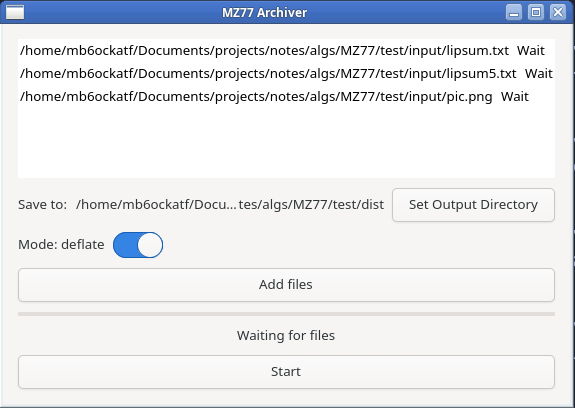
\includegraphics[width=1\textwidth]{pic/test1.png}
\caption{\centering Тестовый запуск 1}
  \label{fig:test1}
\end{figure}
Тестовый запуск архиватора с набором файлов на рис. \ref{fig:test1}.
\begin{figure}[H]
  \centering
  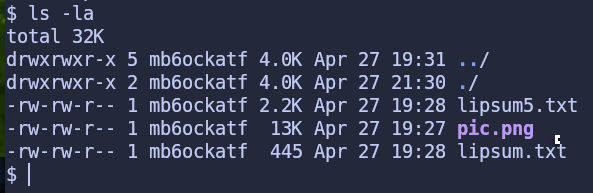
\includegraphics[width=1\textwidth]{pic/test1data.png}
\caption{\centering Размеры файлов в первом тесте}
  \label{fig:test1data}
\end{figure}
Размеры файлов представлены на рис. \ref{fig:test1data}.
\begin{figure}[H]
  \centering
  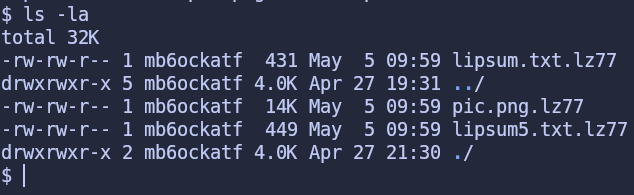
\includegraphics[width=1\textwidth]{pic/test1results.png}
\caption{\centering Размеры результирующих файлов в первом тесте}
  \label{fig:test1results}
\end{figure}
На рис. \ref{fig:test1results} видно, что один файл был сжат более чем в 4
раза. Изображение почти не было сжато из-за недостаточно большого окна
просмотра и малого количества повторяющихся последовательностей байтов.

\begin{figure}[H]
  \centering
  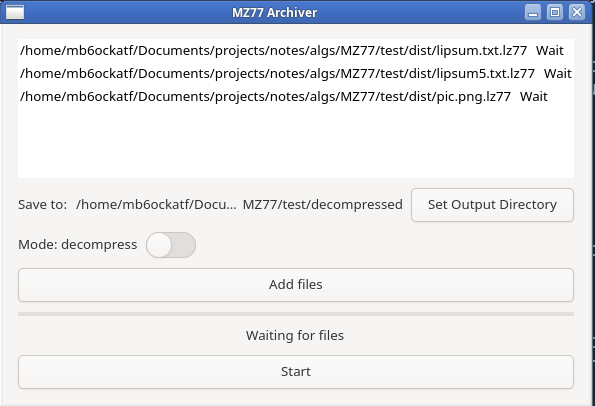
\includegraphics[width=1\textwidth]{pic/test2.png}
\caption{\centering Тестовый запуск 2}
  \label{fig:test2}
\end{figure}
Тестовый запуск архиватора с набором файлов на рис. \ref{fig:test2}. В данном
случае --- распаковка с целью проверки сохранения целостности файлов.

\begin{figure}[H]
  \centering
  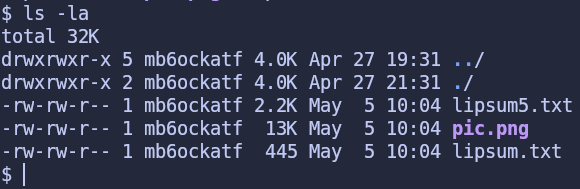
\includegraphics[width=1\textwidth]{pic/test2results.png}
\caption{\centering Размеры результирующих файлов во 2-м тесте}
  \label{fig:test2results}
\end{figure}
На рис. \ref{fig:test2results} видно, что размеры результирующих файлов
совпадают с размерами до архивации.
\begin{figure}[H]
  \centering
  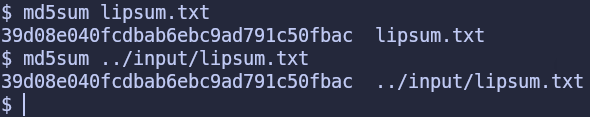
\includegraphics[width=1\textwidth]{pic/check1.png}
\caption{\centering Сохранение целостности первого файла}
  \label{fig:check1}
\end{figure}
\begin{figure}[H]
  \centering
  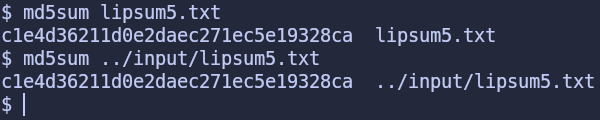
\includegraphics[width=1\textwidth]{pic/check2.png}
\caption{\centering Сохранение целостности 2-го файла}
  \label{fig:check2}
\end{figure}
\begin{figure}[H]
  \centering
  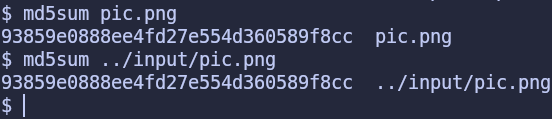
\includegraphics[width=1\textwidth]{pic/check3.png}
\caption{\centering Сохранение целостности 3-го файла}
  \label{fig:check3}
\end{figure}
На рис. \ref{fig:check1}, рис. \ref{fig:check2} и рис. \ref{fig:check3} видно,
что файлы не были повреждены в процессе запаковки и распаковки. Для вычисления
контрольной суммы по алгоритму MD5 была испльзована утилита md5sum из пакета gnu
coreutils.


\newpage
\chapter*{ЗАКЛЮЧЕНИЕ}
\addcontentsline{toc}{chapter}{ЗАКЛЮЧЕНИЕ}
В ходе выполнения курсовой работы был получен опыт работы с многопоточностью,
создания графических интерфейсов на C с помощью возможностей библиотеки
graphical tool kit 4, изучен и реализован алгоритм сжатия LZ77, изучены и
реализованы методы защиты программы от запуска отладчика.

Был получен опыт командной работы над программным продуктом с использованием
пакета git.
\newpage

\newpage
\chapter*{СПИСОК ИСПОЛЬЗОВАННЫХ ИСТОЧНИКОВ}
\addcontentsline{toc}{chapter}{ХОД РАБОТЫ}
\begin{enumerate}
	\item Peter Wright Beginning GTK+/GNOME Programming. - Birmingham: Wrox Press, 2000. - 638 с.
\end{enumerate}

\newpage
\appendix
\renewcommand{\appendixname}{ПРИЛОЖЕНИЕ}
\renewcommand{\thechapter}{\appendixname~\Alph{chapter}} % А, Б, В...

\chapter*{ПРИЛОЖЕНИЕ А}
Листинг 1. Определение хэш-таблицы и её методов.
\begin{verbatim}
typedef struct HashNode {
    DWORD position;
    struct HashNode *next;
} HashNode;

typedef struct {
    HashNode *buckets[HT_SIZE];
} LZHashTable;


static inline uint16_t
hash3 (const uint8_t *p)
{
  return ((uint16_t) p[0] << 10) ^ (p[1] << 4) ^ p[2];
}

\end{verbatim}
\newpage
\chapter*{ПРИЛОЖЕНИЕ B}
Листинг 2. Определение очереди.
\begin{verbatim}
typedef struct {
    enum Mode mode;
    enum TaskStatus status;
    union {
        struct { char in_path[PATH_MAX]; char out_path[PATH_MAX]; } paths;
        struct { size_t original; size_t compressed; double ratio; } stats;
        struct { char msg[256]; } error;
    } data;
} TaskItem;

typedef struct TaskNode {
    TaskItem task;
    struct TaskNode *next;
} TaskNode;


typedef struct {
    TaskNode *head, *tail;
    pthread_mutex_t mutex;
    pthread_cond_t  cond;
    atomic_int count;
    atomic_bool shutdown;
} TaskQueue;
\end{verbatim}

\chapter*{ПРИЛОЖЕНИЕ C}
Листинг 3. Реализация запаковки и распаковки.
\begin{verbatim}
int
lz77_compress (const char *in_path, const char *out_path)
{
  FILE *fin = fopen (in_path, "rb");
  if (!fin)
    return -1;
  FILE *fout = fopen (out_path, "wb");
  if (!fout)
    {
      fclose (fin);
      return -1;
    }
  BitWriter bw;
  bw_init (&bw, fout);
  uint8_t window[WINDOW_SIZE] = { 0 };
  uint32_t ht_heads[HT_SIZE];
  uint32_t ht_next[WINDOW_SIZE];
  memset (ht_heads, 0xFF, sizeof (ht_heads));
  uint8_t buf[WINDOW_SIZE];
  size_t buf_len = fread (buf, 1, sizeof (buf), fin);
  size_t win_pos = 0;
  while (buf_len > 0)
    {
      size_t best_len = 0;
      size_t best_dist = 0;
      if (buf_len >= MIN_MATCH)
	{
	  uint16_t h = hash3 (buf);
	  uint32_t pos = ht_heads[h];
	  while (pos != 0xFFFFFFFF)
	    {
	      if (window[pos % WINDOW_SIZE] == buf[0] &&
		  window[(pos + 1) % WINDOW_SIZE] == buf[1] &&
		  window[(pos + 2) % WINDOW_SIZE] == buf[2])
		{
		  size_t len = 3;
		  while (len < MAX_MATCH && len < buf_len &&
			 window[(pos + len) % WINDOW_SIZE] == buf[len])
		    len++;
		  if (len > best_len)
		    {
		      best_len = len;
		      best_dist = win_pos - pos;
		    }
		}
	      pos = ht_next[pos % WINDOW_SIZE];
	    }
	}
      if (best_len >= MIN_MATCH)
	{
	  bw_write (&bw, 1, 1);
	  bw_write (&bw, (uint32_t) (best_dist - 1), 12);
	  bw_write (&bw, (uint32_t) (best_len - 3), 8);
	  for (size_t i = 0; i < best_len; i++)
	    {
	      window[win_pos % WINDOW_SIZE] = buf[i];
	      if (i + 2 < best_len)
		{
		  uint16_t h = hash3 (&buf[i]);
		  ht_next[win_pos % WINDOW_SIZE] = ht_heads[h];
		  ht_heads[h] = win_pos;
		}
	      win_pos++;
	    }
	  memmove (buf, buf + best_len, buf_len - best_len);
	  buf_len -= best_len;
	}
      else
	{
	  bw_write (&bw, 0, 1);
	  bw_write (&bw, buf[0], 8);
	  window[win_pos % WINDOW_SIZE] = buf[0];
	  if (buf_len >= 3)
	    {
	      uint16_t h = hash3 (buf);
	      ht_next[win_pos % WINDOW_SIZE] = ht_heads[h];
	      ht_heads[h] = win_pos;
	    }
	  win_pos++;
	  memmove (buf, buf + 1, buf_len - 1);
	  buf_len--;
	}
      if (buf_len < sizeof (buf) - 3)
	{
	  size_t rd = fread (buf + buf_len, 1, sizeof (buf) - buf_len, fin);
	  buf_len += rd;
	}
    }
  bw_finish (&bw);
  fclose (fin);
  fclose (fout);
  return 0;
}

int
lz77_decompress (const char *in_path, const char *out_path)
{
  FILE *fin = fopen (in_path, "rb");
  if (!fin)
    return -1;
  FILE *fout = fopen (out_path, "wb");
  if (!fout)
    {
      fclose (fin);
      return -1;
    }
  BitReader br;
  br_init (&br, fin);
  uint8_t window[WINDOW_SIZE] = { 0 };
  size_t win_pos = 0;
  while (1)
    {
      int flag = br_read (&br, 1);
      if (flag == -1)
	break;
      if (flag == 0)
	{
	  int lit = br_read (&br, 8);
	  if (lit == -1)
	    break;
	  fputc ((uint8_t) lit, fout);
	  window[win_pos % WINDOW_SIZE] = (uint8_t) lit;
	  win_pos++;
	}
      else
	{
	  int d_enc = br_read (&br, 12);
	  int l_enc = br_read (&br, 8);
	  if (d_enc == -1 || l_enc == -1)
	    break;
	  uint32_t dist = (uint32_t) d_enc + 1;
	  uint32_t len = (uint32_t) l_enc + 3;
	  uint32_t src = (win_pos + WINDOW_SIZE - dist) % WINDOW_SIZE;
	  for (uint32_t i = 0; i < len; i++)
	    {
	      uint8_t b = window[(src + i) % WINDOW_SIZE];
	      fputc (b, fout);
	      window[(win_pos + i) % WINDOW_SIZE] = b;
	    }
	  win_pos += len;
	}
    }
  fclose (fin);
  fclose (fout);
  return 0;
}
\end{verbatim}

\end{document}
